% !TeX root = Protokoll.tex
\subsection{Grundlagen}

Ein Laser besteht grundlegend aus drei Komponenten, aus dem Lasermedium, einer Pumpquelle und einem Resonator. Das Lasermedium wird mithilfe der Pumpquelle angeregt und emittiert Licht, durch den Resonator wird dies verstärkt. Dieser Aufbau hat den Vorteil, dass das Licht monochromatisch ist, mit hoher Intensität und Kohärenz.
\subsection{Zwei Niveau Laser}
\begin{figure}
\centering
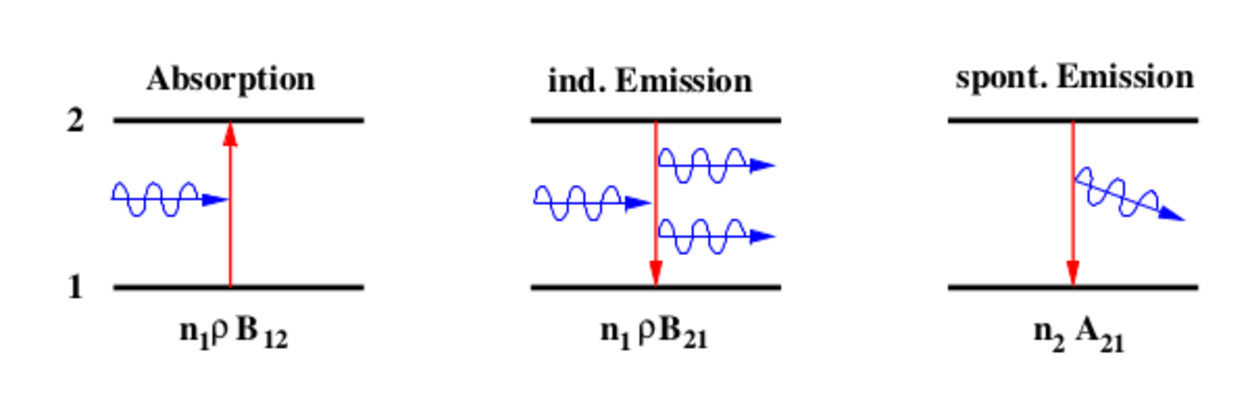
\includegraphics[scale=0.75]{../Grafiken/Emission.pdf}
\caption{Eine Veranschaulichung der Funktionsweise eines zwei Niveau Lasers\cite{V61}\label{Emission}}
\end{figure}
Der einfachste theoretische Laser, ist wenn das Lasermedium  zwei Niveaus besitzt. Die Besetzungszahlen werden mit $n_1$ für das Grundniveau und $n_2$ für den angeregten Zustand bezeichnet. Durch ein Photon, mit der Energie des Übergangs, wird es Absorbiert und das System geht in den angeregten Zustand über.\\
Vom angeregten Zustand kann es durch spontane oder induzierten Emission zurück in den Grundzustand. Die Kohärenz wird durch die stimulierte Emission erreicht. Dabei löst ein Photon ein weiteres aus dem System, das dann wieder in den Grundzustand übergeht. Das ausgelöste Photon hat die Selbe Energie, Phase und Ausbreitungsrichtung, wie das Photon welches es ausgelöst hat. Wird nun ein Strahlenfeld $\rho$ angelegt, so wird durch Wechselwirkung die Besetzungsdichte $n_2$ durch Emission verringert und durch Absorption erhöht.
Die Änderung der Photonenanzahl in einem Volumen wird gegeben durch
\begin{align}
\dot{N}_A&=n_1 \rho B_{12}\\
\dot{N}_{IE}&=n_2\rho B_{21}\\
\dot{N}_{SE}&=n_2A_{21},
\end{align} dabei ist $\dot{N}_A$ die Änderung der Photonen durch Absorption, $\dot{N}_{IE}$ die Änderung der Photonen durch induzierte Emission und $\dot{N}_{SE}$ die Änderung durch Spontane Emission. Die Konstanten $A_{21}$, $B_{12}$ und $B_{21}$ sind die Einsteinkoeffizienten und geben die Übergangswahrscheinlichkeiten an.\\
Unter der Annahme das keine Verluste auftreten, also die Summe von $n_1$ und $n_2$ konstant ist, ergeben sich die Ratengleichungen als
\begin{align}
\frac{dn_1}{dt}=&-n_1 \rho B_{12} + n_2\rho B_{21} + n_2 A_{21}\\
\frac{dn_2}{dt}=&+n_1\rho B_{12} - n_2\rho B_{21} -n_2A_{21}.
\end{align}Damit der Strahl des Lasers dauerhaft kohärent bleibt, müssen die höheren Niveaus mehr besetzt sein als das Grundniveau, dadurch tritt spontane Emission seltener als induzierte Emission auf, dies wird als Besetzungsinversion bezeichnet.
Ein zwei Niveau Laser ist nicht möglich. Wenn beide Zustände gleich viel besetzt sind, ist die Wahrscheinlichkeit das ein Photon durch stimulierte Emission emittiert wird, genauso groß wie das ein Photon absorbiert wird, zusätzlich werden Photonen immer noch durch spontane Emission emittiert. 
\subsection{Stabilität eines Lasers}
\begin{figure}[h!]
\centering
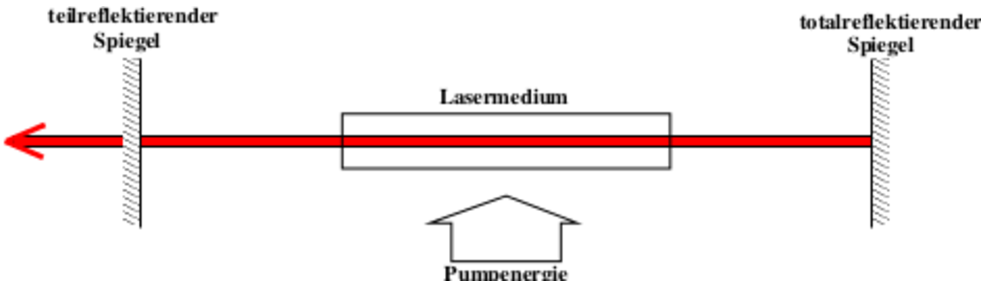
\includegraphics[scale=0.75]{../Grafiken/Laser.pdf}
\caption{Die Skizze eines Lasers\cite{V61}\label{SkizzeLaser}}
\end{figure}
 Um den Zustand der Besetzungsinversion zu erzeugen und aufrecht zu erhalten, muss mithilfe der Pumpquelle, dem Lasermedium dauerhaft Energie hinzugefügt werden. Dies geschieht durch Elektronenstöße oder optische Anregung. Durch einen optischen Resonator wird die Strecke, die der Strahl zur Anregung, durch das Lasermedium zurücklegt maximiert.\\
Einer der beiden Resonatorspiegel ist teildurchlässig, dadurch wird ein Teil des Strahls aus gekoppelt. Die Verluste durch die Resonatorspiegel müssen minimal gehalten werden, durch konfokale Spiegel deren Brennpunkte aufeinander Fallen, ist dies der Fall.\\
Sind die Verstärkung durch die induzierte Emission größer als die Verluste durch die Resonatorspiegel, dann ist der Resonator stabil. Dann wird
\begin{align}
0\le g_1\cdot g_2 < 1
\end{align}
erfüllt, dabei ist der Resonatorparameter $g_i=1-L/r_i$ und $L$ die Resonatorlänge und $r_i$ der Krümmungsradius des jeweiligen Spiegels. Die Stabilität ist somit nicht nur von dem Typ des Resonators sondern auch von dem Krümmungsradius der Spiegel abhängig.
\begin{figure}
\centering
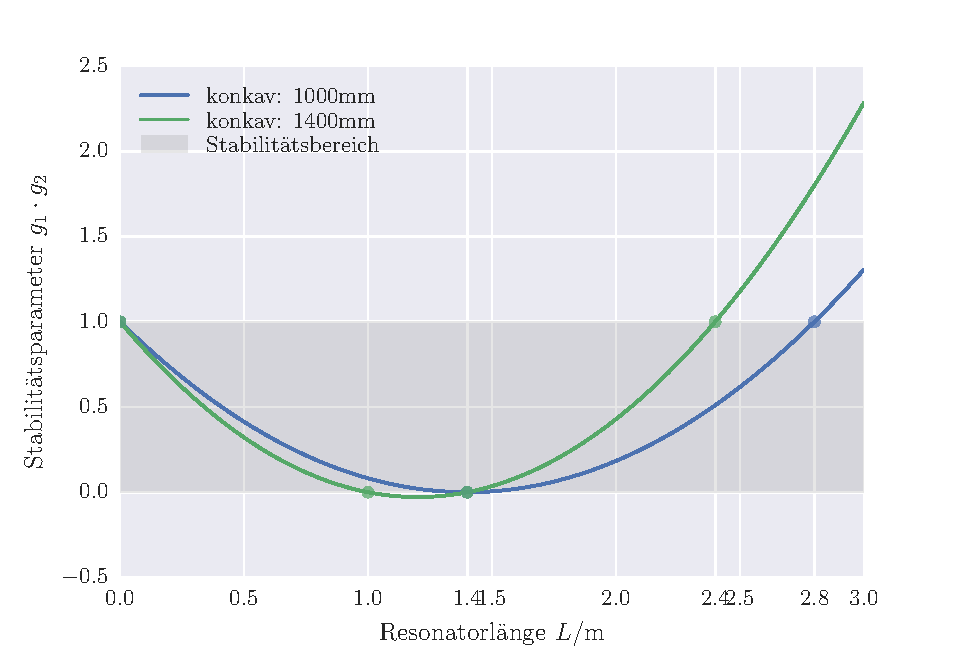
\includegraphics[scale=0.75]{../Grafiken/Stabilitaetsparameter.pdf}
\caption{Plot der Stabilitätsbedingung für zwei der zur Verfügung stehenden Spiegel, siehe Tabelle \ref{Eigenschaften}}
\label{fig:Stabilitaet}
\end{figure}
\subsection[TEM-Moden]{$\mathbf{TEM}$-Moden}
Innerhalb des Resonators befinden sich $q$ Wellenlängen die sich longitudinal ausbreiten, weil die Resonatorlänge $L$ um einiges größer ist als die Wellenlänge $\lambda$, $q$ wird auch die longitudinale Mode genannt. Aufgrund von Unebenheiten oder Verkippung des Spiegels entstehen auch transversale Moden $l$ und $p$ die für die $x-$ und $y-$Richtungne stehen. Daraus ergibt sich $\mathrm{TEM}_{lpq}$-Moden (transverse electromagnetic Mode), die als Anlehnung an den Hohlleiter verwendet wird. Die Modenzahl $q$ kann weggelassen werden weil sie von keiner Bedeutung ist. In den meisten Resonatoren werden nur wenige Moden isoliert und verstärkt.\\

Die Grundmode $\mathrm{TEM}_{00}$ ist die Mode mit der höchsten Symmetrie und den wenigsten Verlusten. Die Intensität von der Mode wird durch die Gaußverteilung beschrieben.
\begin{align}
I(r)=I_0\exp\left(\frac{-2r^2}{\omega^2}\right)
\label{eq:tem00}
\end{align}
Hier ist $I_0$ die Maximalintensität, $r$ der Abstand zur optischen Achse und $\omega$ der Strahlenradius. Der Strahlenradius lässt sich durch
\begin{align}
\omega(z)=\omega_0 \sqrt{1+\left(\frac{\theta z}{\omega_0}\right)^2}
\end{align}
beschreiben, dabei ist $\omega_0$ der minimale Strahltaille, $z$ der Abstand auf der optischen Achse und $\theta$ die Strahlendivergenz, wie durch die Gaußsche 
Strahlenoptik beschrieben.
Unter der Annahme die verwendeten Spiegel seien sphärisch, erhält man für die erste transversale Mode $\mathrm{TEM}_{10}$ 
die Intensitätsverteilung durch Multiplikation der Grundmodenverteilung mit dem Quadrat des ersten Hermiteschen Polynom\footnotemark $H_1\qty(\sqrt{2}\frac{r}{\omega})$\cite{Demtroeder07}
zu
\begin{align}
I(r)=I_0\frac{8r^2}{\omega^2}\exp\left(\frac{-2r^2}{\omega^2}\right).
\label{eq:tem10}
\end{align}
Folgend werden weitere Formel diskutiert die für die Auswertung benötigt werden.
Die Abhängigkeit der Laserintensität von dem Winkel $\phi$, der am Polarisator eingestellt wurde, ist durch
\begin{align}
I(\phi)=I_0\sin[2](\phi - \phi_0)
\label{eq:polarisation}
\end{align}
beschrieben. 
Die Wellenlänge des Laserlichts lässt sich mit Hilfe von Beugung am Gitter und der Gleichung
\begin{align}
\lambda=\frac{g}{n}\sin\left(  \theta \right)
\label{eq:gitter}
\end{align}
berechnen, dabei ist $g$ der Gitterabstand, $n$ die Nummer des Maxima und $\theta$ der Winkel zwischen der optischen Achse und dem Maxima. Dieser Winkel wird bestimmt durch den Abstand vom Gitter zum Hauptmaximum $l$ und dem Abstand vom  Hauptmaximum zum Nebenmaximum $d$ durch
\begin{align}
\frac{d}{l}=\tan\left( \theta \right).
\label{eq:gitter_winkel}
\end{align}


\footnotetext{Das erste Hermitesche Polynom ist $H_1(x) = 2x$.}

\subsection{Der HeNe-Laser}
Der HeNe-Laser gehört zu den Gaslasern und das Gemisch aus Helium und Neon hat ein Verhältnis von 5 zu 1. Innerhalb der Laserrohrs befindet sich ein Druck von 1 Torr.Dabei fungiert Helium als Pumpquelle und Neon als Lasermedium. Durch elektrische Entladung wird das Helium in den angeregten Zustand versetzt und gibt die Anregungsenergie durch Stöße zweiter Ordnung an das Neon ab, dadurch wird Besetzungsinversion erzeugt. Der Laser besitzt die intensivste Wellenlänge bei $\lambda=$632,8 nm.
Die Polarisation des Lasers wird mithilfe von Brewster-Fenstern erreicht, diese Fenster stehen im Brewster-Winkel zur Strahlenachse, was dafür sorgt, dass alle Polarisationen  bis auf das parallel zur Einfallsebene komplett reflektiert wird und so mit aus dem System entfernt wird.
